\documentclass{beamer}

% Use the UiB theme
\usetheme{UiB}
% For strikethrough text using \sout
\usepackage[normalem]{ulem}

% For figures
\usepackage{graphicx}
\usepackage{tikz}
\usetikzlibrary{shapes.geometric,positioning,shapes.symbols,overlay-beamer-styles}

\usepackage{listings}
\usepackage{xcolor}
\usepackage{color}
\usepackage{generators/listings-golang}
\usepackage{generators/listings-haskell}
\usepackage{generators/listings-magnolia}
\usepackage{generators/listings-typescript}
\usepackage{amsmath}

% Presentation metadata
\title{Developing a zero-core modular IDE}
\subtitle{Creating a zero-cost IDE; you get what you pay for}
\author{Nils Michael Fitjar}
\institute{University of Bergen}
\date{\today}

\begin{document}
\section{Introduction}
\SectionPage

% NOTE: This is a vague simili on software development and building a house,
% specifically pointing out how _rigorus_ development and builiding is, as most
% developers do not take into account of changing priorities when developing.
\begin{frame}
  \frametitle{Software development}
  \begin{itemize}
    \item Like building a house
    \pause
    \begin{itemize}
      \item Strong foundation
      \pause
      \item Built for a purpose
      \pause
      \item Renovations/remodeling is expensive
      \pause
    \end{itemize}
    \item Change of:
    \pause
    \begin{itemize}
      \item Guards
      \pause
      \item Scope
      \pause
      \item Priorities
      \pause
    \end{itemize}
    \item Leads to an expensive refactoring
    \pause
    \item Or expensive rebuilding
    \pause
    \item A concrete example is an IDE
  \end{itemize}
\end{frame}

\begin{frame}
  \frametitle{The Solution To The Problem}
  \begin{quote}
    "It works on my machine." \textemdash Intern
  \end{quote}
  \begin{itemize}
    \item The text editor, the compiler, and the terminal,
    \pause
    \item Eventually needed build scripts for large projects
    \pause
    \begin{itemize}
      \item Lead to more complex build scripts
      \pause
      \item Eventually ending up with applications like Gradle and Maven
      \pause
    \end{itemize}
    \item Missing/incomplete:
    \pause
    \begin{itemize}
      \item Libraries
      \pause
      \item Environment variables
      \pause
      \item Configurations
      \pause
      \item Scripts
      \pause
    \end{itemize}
  \item What if everything is bundled?
  \end{itemize}
\end{frame}

\begin{frame}
  \frametitle{Integrated Development Environment}
  \begin{itemize}
    \item Easier to onboard new developers
    \pause
    \item Other quality of life improvements
    \pause
    \begin{itemize}
      \item File explorer
      \pause
      \item Project manager
      \pause
      \item Version Control System integration
      \pause
      \item Syntax Highlighting
      \pause
      \item Integrated debugging
      \pause
      \item \dots
    \end{itemize}
  \end{itemize}
\end{frame}

\section{Who cares?}
\SectionPage

\begin{frame}
  \frametitle{Bergen Language Design Laboratory}
  \begin{itemize}
    \item Experimenting with a research programming language called Magnolia
    \pause
    \item Takes inspiration from
    \pause
    \begin{itemize}
      \item Generic programming
      \pause
      \item Algebraic specifications
      \pause
      \item Theory of institutions
      \pause
      \item And other languages like CafeOBJ and Maude
      \pause
    \end{itemize}
    \item Created to experiment with novel language features
    \begin{itemize}
      \item Functionalization
      \pause
      \item Mutification
      \pause
      \item Generated types
      \pause
      \item Type partitions
      \pause
      \item \dots
    \end{itemize}
  \end{itemize}
\end{frame}

\begin{frame}
  \frametitle{Magnolia}
  \begin{itemize}
    \item Introduces something called \textit{concepts}
    \pause
    \item Similar to an Java interface.
    \pause
    \item A concept declares
    \begin{itemize}
      \item Types
      \pause
      \item Operations on those types
      \pause
      \item Axioms that specify the behavior of the operations
      \pause
    \end{itemize}
    \item A concept can use other concepts, and rename the types and operations
      in the concept, this is called renaming
  \end{itemize}
\end{frame}

\begin{frame}
  \frametitle{Magma example in mathematical notation}
  \begin{itemize}
    \item Magma
    \begin{itemize}
      \item Set $M$
      \item Binary operation $\bullet$
      \begin{equation}
        \forall a, \forall b \in M \implies a \bullet b \in M
      \end{equation}
    \end{itemize}
  \end{itemize}
\end{frame}

\begin{frame}
    \frametitle{Magma example in Java}
    \begin{center}
      \lstinputlisting
      [ language=Java
      ]{./code/magma.java}
    \end{center}
\end{frame}

\begin{frame}
    \frametitle{Magma example in Magnolia}
    \begin{center}
      \lstinputlisting
      [ language=Magnolia
      ]{./code/magma.mg}
    \end{center}
\end{frame}

\begin{frame}
  \frametitle{Semigroup example in mathematical notation}
  \begin{itemize}
    \item Semigroup
    \begin{itemize}
      \item Set $M$
      \item Binary operation $\bullet$
      \begin{equation}
       \forall a, \forall b \in M \implies a \bullet b \in M
      \end{equation}
      \begin{equation}
        \forall a, \forall b, \forall c \in M \implies
        (a \bullet b) \bullet c = a \bullet (b \bullet c)
      \end{equation}
    \end{itemize}
  \end{itemize}
\end{frame}

\begin{frame}
    \frametitle{Semigroup example in Java}
    \begin{center}
      \lstinputlisting
      [ language=Java
      ]{./code/semigroup.java}
    \end{center}
\end{frame}

\begin{frame}
    \frametitle{Semigroup example in Magnolia}
    \begin{center}
      \lstinputlisting
      [ language=Magnolia
      ]{./code/semigroup.mg}
    \end{center}
\end{frame}

\begin{frame}
  \frametitle{Monoid example in mathematical notation}
  \begin{itemize}
    \item Monoid
    \begin{itemize}
      \item Set $M$
      \item Binary operation $\bullet$
      \begin{equation}
       \forall a, \forall b \in M \implies a \bullet b \in M
      \end{equation}
      \begin{equation}
        \forall a, \forall b, \forall c \in M \implies
        (a \bullet b) \bullet c = a \bullet (b \bullet c)
      \end{equation}
      \begin{equation}
        \forall a, \exists e \in M \implies a \bullet c = a
      \end{equation}
    \end{itemize}
  \end{itemize}
\end{frame}

\begin{frame}
    \frametitle{Monoid example in Java}
    \begin{center}
      \lstinputlisting
      [ language=Java
      ]{./code/monoid.java}
    \end{center}
\end{frame}

\begin{frame}
    \frametitle{Monoid example in Magnolia}
    \begin{center}
      \lstinputlisting
      [ language=Magnolia
      ]{./code/monoid.mg}
    \end{center}
\end{frame}

\begin{frame}
  \frametitle{Group example in mathematical notation}
  \begin{itemize}
    \item Group
    \begin{itemize}
      \item Set $M$
      \item Binary operation $\bullet$
      \begin{equation}
       \forall a, \forall b \in M \implies a \bullet b \in M
      \end{equation}
      \begin{equation}
        \forall a, \forall b, \forall c \in M \implies
        (a \bullet b) \bullet c = a \bullet (b \bullet c)
      \end{equation}
      \begin{equation}
        \forall a, \exists e \in M \implies a \bullet e = a
      \end{equation}
      \begin{equation}
        \forall a, \exists b \in M \implies a \bullet b = e
      \end{equation}
    \end{itemize}
  \end{itemize}
\end{frame}

\begin{frame}
    \frametitle{Group example in Java}
    \begin{center}
      \lstinputlisting
      [ language=Java
      ]{./code/group.java}
    \end{center}
\end{frame}

\begin{frame}
    \frametitle{Group example in Magnolia}
    \begin{center}
      \lstinputlisting
      [ language=Magnolia
      ]{./code/group.mg}
    \end{center}
\end{frame}

\begin{frame}
  \frametitle{If It Ain't Broke}
  The current Magnolia IDE
  \pause
  \begin{itemize}
    \item Integrated with the Magnolia Compiler
    \pause
    \item Made using an old version of Eclipse
    \pause
    \item Uses deprecated Eclipse plugins
    \pause
    \item Installation process is complex
    \pause
    \item In INF220, two weeks is set aside for students to install it
  \end{itemize}
\end{frame}

\section{Why create a \textit{new} IDE?}
\SectionPage

\begin{frame}
  \frametitle{Forking VS Code And Adding AI}
  \begin{itemize}
    \item Current IDEs cannot have good support for all experimental programming
      languages
      \pause
      \begin{itemize}
        \item So niche solutions are needed
          \pause
        \item Which might depend on very specific functionality from the host
          IDE
          \pause
      \end{itemize}
    \item The host IDE could deprecate needed functionality
      \pause
    \item The installation process would then be complex
      \pause
    \item Deep understanding of the host IDE is needed
  \end{itemize}
\end{frame}

\begin{frame}
  \frametitle{Why Modular?}
  \begin{itemize}
    \item Magnolia is still in development
      \pause
    \item The Magnolia toolchain is being developed in parallel
      \pause
    \item Modularity allows for future discoveries to be quickly adopted into
      the IDE
      \pause
    \item Lowers the onboarding time for future maintainers
  \end{itemize}
\end{frame}


\section{Planning a zero-core modular IDE}
\SectionPage

\begin{frame}
  \frametitle{What is a module?}
  \begin{itemize}
    \item Third party code to be executed/interpreted
      \pause
      \begin{itemize}
        \item Tailor made scripting language
          \pause
          \begin{itemize}
            \item Vim Script (Vim)
              \pause
          \end{itemize}
        \item An already existing programming language
          \pause
          \begin{itemize}
            \item Lua (NeoVim)
              \pause
            \item JavaScript (VS Code)
              \pause
            \item Java/Kotlin/Clojure (Eclipse/IntelliJ)
          \end{itemize}
      \end{itemize}
  \end{itemize}
\end{frame}

\begin{frame}
  \frametitle{Features \& Goals}
  \begin{itemize}
    \item Easy to extend (with modules)
      \pause
      \begin{itemize}
        \item Low bar to create a module
          \pause
        \item Easy to reason about how modules work together
      \end{itemize}
    \item Simple installation, for multiple OSes
      \pause
    \item Modular core
      \pause
    \item Good module developer experience
      \begin{itemize}
          \pause
        \item Language agnostic module architecture
          \pause
        \item Good debugging tools
          \pause
        \item Good module library
      \end{itemize}
  \end{itemize}
\end{frame}

\section{Modeling a module}
\SectionPage

\begin{frame}
  \frametitle{How To model a module?}
  \begin{itemize}
    \item A module needs to:
      \pause
      \begin{itemize}
        \item Initialize some state
        \pause
        \item Update the state based on events
        \pause
        \item Change the view based on the state
      \end{itemize}
      \pause
    \item Module architecture is inspired by Elm and MVC
      \pause
    \item A module should be \textit{pure}
  \end{itemize}
\end{frame}

\hidelogo

\begin{frame}
  \frametitle{Scrapped architecture}
  \begin{figure}
    \centering
    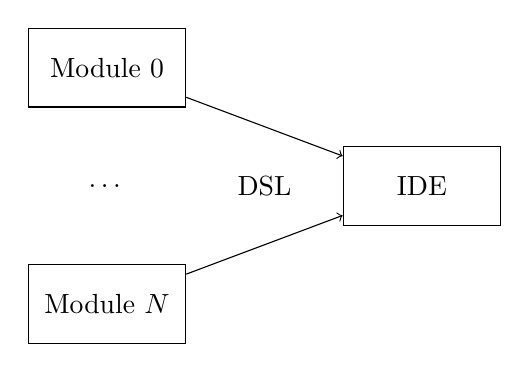
\begin{tikzpicture}
  % Nodes
  \node (p0) [rectangle, draw, minimum height=1cm, minimum width=2cm] at (0, 1.5) {Module 0};
  \node (dots) [] at (0, 0) {\dots};
  \node (dsl) [] at (2, 0) {DSL};
  \node (p1) [rectangle, draw, minimum height=1cm, minimum width=2cm] at (0, -1.5) {Module $N$};
  \node (i) [rectangle, draw, minimum height=1cm, minimum width=2cm] at (4, 0) {IDE};
  % Arrow
  \draw[<-] (i) to node[midway, above] {} (p0);
  \draw[<-] (i) to node[midway, above] {} (p1);
  % Header
\end{tikzpicture}
    \caption{DSL inspired module architecture}
  \end{figure}
\end{frame}

\begin{frame}
  \frametitle{Scrapped architecture}
  \begin{figure}
    \centering
    \begin{minted}{haskell}
-- Manifest :: Map
init :: Map
init :: [("counter", ValInt 0)]

update :: Msg -> Map -> Map
update (PluginMsg "counter") model =
  case lookup "counter" model of
    Just (ValInt i) -> insert "counter" (ValInt (i + 1)) model
    Nothing -> insert "counter" (ValInt 0) model

view :: Map -> Html
view model = Div [] [Text "Hello, World!"
  , Btn [OnClick (PluginMsg "counter")] []
  , Text (putStrLn (lookupOrDefault "counter" model))
\end{minted}



    \caption{Elm inspired module architecture}
  \end{figure}
\end{frame}

\begin{frame}
  \frametitle{Current architecture}
  \begin{figure}
    \centering
    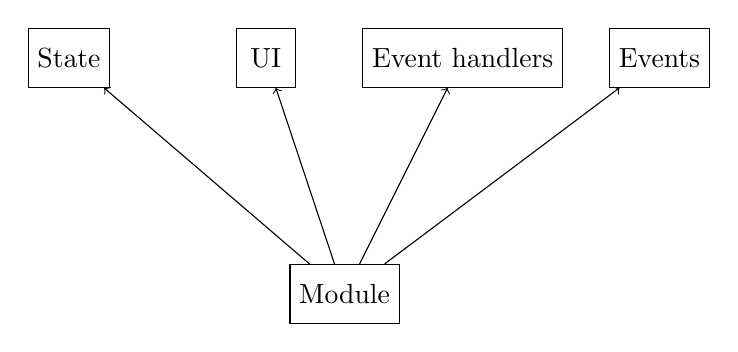
\begin{tikzpicture}
  % Nodes
  \node (state) [rectangle, draw, minimum height=0.75cm, minimum width=1cm] at (-3.5, 0) {State};
  \node (ui) [rectangle, draw, minimum height=0.75cm, minimum width=0.75cm] at (-1, 0) {UI};
  \node (eventH) [rectangle, draw, minimum height=0.75cm, minimum width=0.75cm] at (1.5, 0) {Event handlers};
  \node (event) [rectangle, draw, minimum height=0.75cm, minimum width=0.75cm] at (4, 0) {Events};
  \node (module) [rectangle, draw, minimum height=0.75cm, minimum width=0.75cm] at (0, -3) {Module};
  % Arrow
  \draw[->] (module) to[] node[midway, above] {} (ui);
  \draw[->] (module) to[] node[midway, above] {} (state);
  \draw[->] (module) to[] node[midway, above] {} (event);
  \draw[->] (module) to[] node[midway, above] {} (eventH);
  %\draw[->] (p) to[out=60, in=120] node[midway, above] {Html/State} (i);
  %\draw[->] (i) to[out=-120, in=-60] node[midway, above] {Msg/State} (p);
  % Header
\end{tikzpicture}

    \caption{Initialization stage}
  \end{figure}
\end{frame}


\begin{frame}
  \frametitle{Current Architecture}
  \begin{figure}
    \centering
    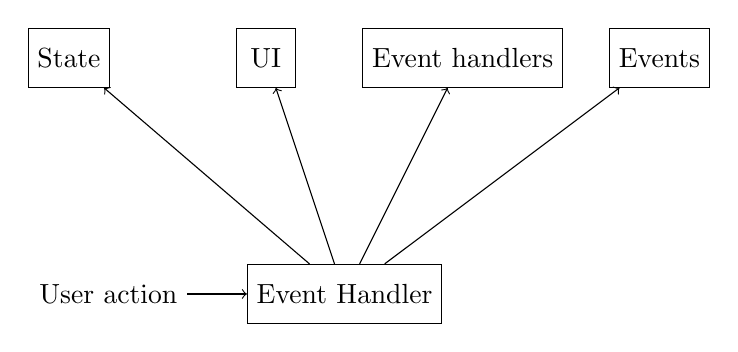
\begin{tikzpicture}
  % Nodes
  \node (state) [rectangle, draw, minimum height=0.75cm, minimum width=1cm] at (-3.5, 0) {State};
  \node (ui) [rectangle, draw, minimum height=0.75cm, minimum width=0.75cm] at (-1, 0) {UI};
  \node (eventH) [rectangle, draw, minimum height=0.75cm, minimum width=0.75cm] at (1.5, 0) {Event handlers};
  \node (event) [rectangle, draw, minimum height=0.75cm, minimum width=0.75cm] at (4, 0) {Events};
  \node (module) [rectangle, draw, minimum height=0.75cm, minimum width=0.75cm] at (0, -3) {Event Handler};
  \node (event0) [] at (-3, -3) {User action};
  % Arrow
  \draw[->] (module) to[] node[midway, above] {} (ui);
  \draw[->] (module) to[] node[midway, above] {} (state);
  \draw[->] (module) to[] node[midway, above] {} (event);
  \draw[->] (module) to[] node[midway, above] {} (eventH);
  \draw[->] (event0) to[] node[midway, above] {} (module);
  %\draw[->] (p) to[out=60, in=120] node[midway, above] {Html/State} (i);
  %\draw[->] (i) to[out=-120, in=-60] node[midway, above] {Msg/State} (p);
  % Header
\end{tikzpicture}

    \caption{Post initialization stage}
  \end{figure}
\end{frame}

\showlogo

\section{Implementation struggles}
\SectionPage

\begin{frame}
  \frametitle{I need super computer time for my featureless app}
  \begin{itemize}
    \item When implementing the Elm inspired module architecture
    \pause
    \item \textit{Basic} module, which should only display "Hello, World!"
    \pause
      \begin{figure}
        \centering
        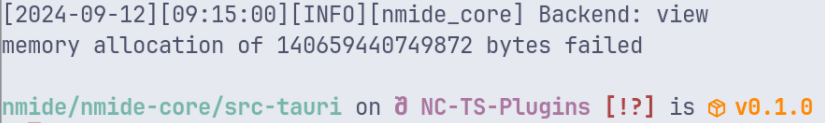
\includegraphics[width=0.9\textwidth]{./pics/memory-allocation-zoomed.png}
        \caption{140.6594 Terabytes of memory}
      \end{figure}
  \end{itemize}
\end{frame}

\hidelogo

\showlogo
\begin{frame}
  \frametitle{Module V.1 - Final.Final}
  \begin{itemize}
    \item Everything* is a module
      \pause
    \item Modules can \textit{invoke} modules
      \pause
    \begin{itemize}
      \item Init - Returns a set of modifications
    \end{itemize}
    \pause
    \item Pros
    \pause
    \begin{itemize}
      \item Modular
        \pause
      \item Modules can \textit{invoke} other modules
    \end{itemize}
    \pause
    \item Cons
    \begin{itemize}
        \pause
      \item Complex to implement
    \end{itemize}
  \end{itemize}
\end{frame}

\begin{frame}
  \frametitle{Module Architecture}
  \begin{figure}
    \centering
    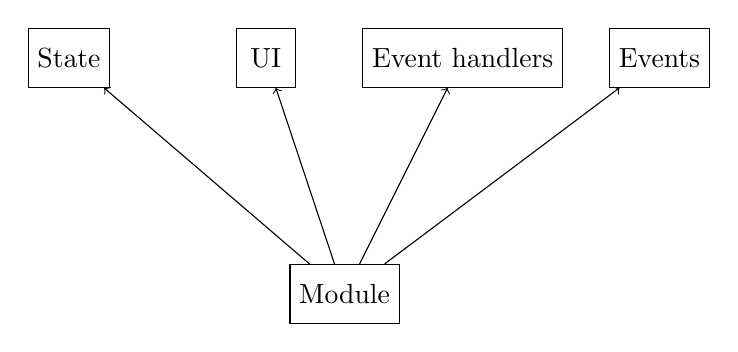
\begin{tikzpicture}
  % Nodes
  \node (state) [rectangle, draw, minimum height=0.75cm, minimum width=1cm] at (-3.5, 0) {State};
  \node (ui) [rectangle, draw, minimum height=0.75cm, minimum width=0.75cm] at (-1, 0) {UI};
  \node (eventH) [rectangle, draw, minimum height=0.75cm, minimum width=0.75cm] at (1.5, 0) {Event handlers};
  \node (event) [rectangle, draw, minimum height=0.75cm, minimum width=0.75cm] at (4, 0) {Events};
  \node (module) [rectangle, draw, minimum height=0.75cm, minimum width=0.75cm] at (0, -3) {Module};
  % Arrow
  \draw[->] (module) to[] node[midway, above] {} (ui);
  \draw[->] (module) to[] node[midway, above] {} (state);
  \draw[->] (module) to[] node[midway, above] {} (event);
  \draw[->] (module) to[] node[midway, above] {} (eventH);
  %\draw[->] (p) to[out=60, in=120] node[midway, above] {Html/State} (i);
  %\draw[->] (i) to[out=-120, in=-60] node[midway, above] {Msg/State} (p);
  % Header
\end{tikzpicture}

  \end{figure}
\end{frame}

\begin{frame}
  \frametitle{Module Type}
  \begin{center}
    \lstinputlisting
    [ language=Haskell
    ]{./code/module-example.hs}
  \end{center}
\end{frame}


\begin{frame}
  \frametitle{Event Type}
  \begin{center}
    \lstinputlisting
    [ language=Haskell
    ]{./code/module-example-event.hs}
  \end{center}
\end{frame}


\section{Modules}
\SectionPage

\begin{frame}
  \frametitle{Event sender}
\end{frame}

\begin{frame}
  \frametitle{Cache}
\end{frame}

\begin{frame}
  \frametitle{Editor}
\end{frame}

\begin{frame}
  \frametitle{Error reporting}
\end{frame}

\begin{frame}
  \frametitle{File explorer}
\end{frame}

\begin{frame}
  \frametitle{File icons}
\end{frame}

\begin{frame}
  \frametitle{UI framework}
\end{frame}

\begin{frame}
  \frametitle{File system operations}
\end{frame}

\begin{frame}
  \frametitle{Tabs}
\end{frame}

\begin{frame}
  \frametitle{Magnolia dependency graph}
\end{frame}

\begin{frame}
  \frametitle{Module installer}
\end{frame}

\begin{frame}
  \frametitle{State visualization}
\end{frame}

\begin{frame}
  \frametitle{Rust dependencies}
\end{frame}

%\hidelogo

\begin{frame}
  \frametitle{Module dependency viewer}
\end{frame}

\begin{frame}
  \frametitle{Module dependencies}
  \begin{figure}
    \centering
      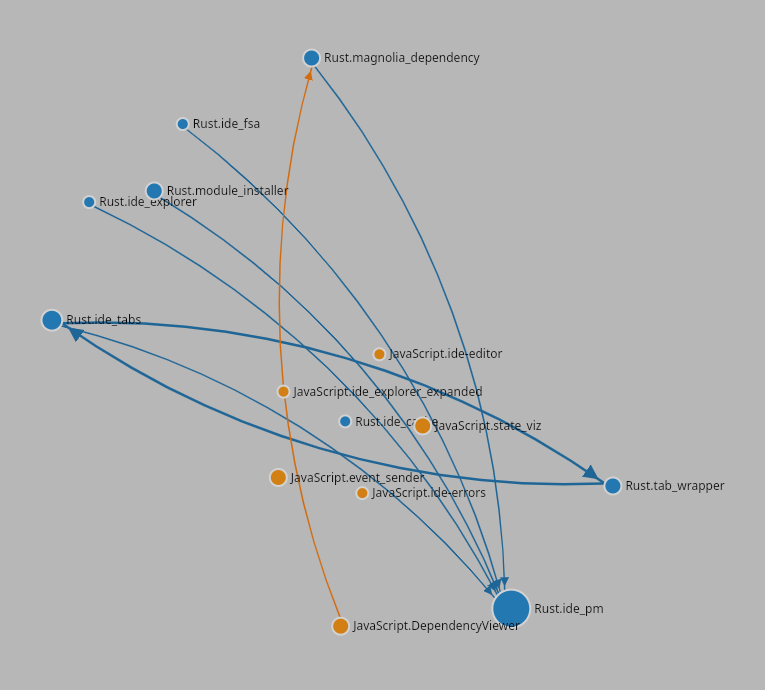
\includegraphics[width=0.7\textwidth]{./pics/module-dependencies.png}
  \end{figure}
\end{frame}

%\showlogo


\section{Conclusion}
\SectionPage

\begin{frame}
  \frametitle{Development process}
  \begin{itemize}
    \item Developed using modern development techniques
    \pause
    \begin{center}
      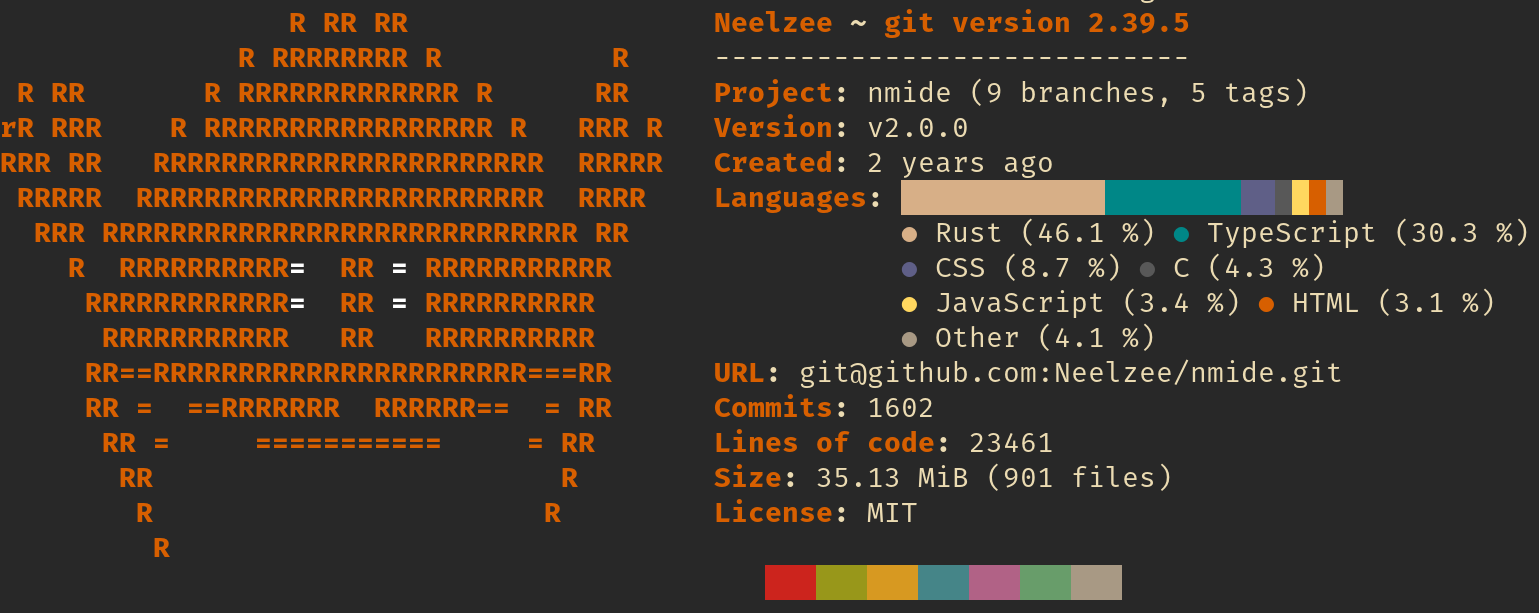
\includegraphics[width=0.8\textwidth]{./pics/onefetch.png}
    \end{center}
  \end{itemize}
\end{frame}

\begin{frame}
  \frametitle{Testing}
  \begin{itemize}
    \item Tests for the Rust libraries
    \pause
    \begin{center}
      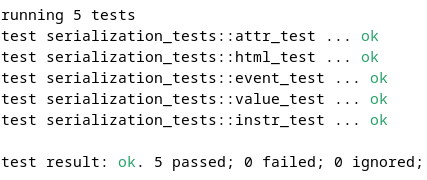
\includegraphics[width=0.45\textwidth]{./pics/librstest.png}
    \end{center}
    \pause
    \item Tests for the JavaScript libraries
    \pause
    \begin{center}
      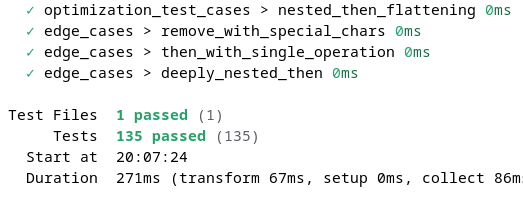
\includegraphics[width=0.45\textwidth]{./pics/libtest.png}
    \end{center}
  \end{itemize}
\end{frame}

\begin{frame}
  \frametitle{Goals}
  \pause
  \begin{itemize}
    \item All functionality comes from modules
    \pause
    \item Modules can be made in different programming languages
    \pause
    \item The core can only load modules
    \pause
    \item Allows for blocking or non-blocking threading
    \pause
    \item The core is modular
    \pause
    \begin{itemize}
      \item Can be run as a web IDE
    \end{itemize}
  \end{itemize}
\end{frame}

\section{Demo}
\SectionPage

\end{document}
